% \documentclass[11pt]{article} 
% \usepackage{cmap} 
% \usepackage{graphicx}
% \usepackage[T2A]{fontenc}
% \usepackage[russian]{babel} 
% \usepackage[utf8]{inputenc} 
% \usepackage{amsmath, amssymb}
% \usepackage{tabularx}
% \usepackage{hologo}
% \usepackage{hyperref}
% \usepackage{bbm}
% \usepackage{wasysym}
% \usepackage[pdftex]{graphicx}
% \def\multiset#1#2{\ensuremath{\left(\kern-.3em\left(\genfrac{}{}{0pt}{}{#1}{#2}\right)\kern-.3em\right)}}
% % \title{История одной моральной дилеммы}
% % \author{Захаров Владимир Олегович}
% % \date{}
% \begin{document}
% % \maketitle
% % Давай представим следующую ситуацию: Иван делает Марии предложение, но та отказывает ему, в ответ на что Иван угрожает покончить с собой. Мария не воспринимает эти слова всерьез, но Иван все же накладывает на себя руки, в предсмертной записке обвиняя во всем Марию. Оправданно ли он это делает? Несет ли Мария моральную ответственность за смерть Ивана? Попробуем разобраться в этом.
% % \par
% % Ситуация, в которой Мария отказывает Ивану на его предложение, после чего он совершает суицид, поднимает важные вопросы о морали, свободе воли и ответственности. Оправдано ли обвинение Марии в предсмертной записке Ивана? Несет ли она ответственность за его смерть? Чтобы проанализировать эту дилемму, обратимся к концепциям свободы воли, деонтологии и утилитаризма, рассматривая их взгляды на моральную ответственность и обязательства.
% % \par
% % Свобода воли тесно связана с понятием моральной ответственности. Согласно компатибилизму, человек может быть морально ответственным за свои действия, даже если его поступки детерминированы обстоятельствами, и он не мог бы поступить иначе. Гарри Франкфурт в своих работах утверждает, что, хотя внешние условия могут ограничивать свободу выбора, человек несет ответственность, если его действия совпадают с его истинными желаниями и намерениями (то есть желания первого порядка совпадают с желаниями второго порядка). В случае с Иваном его решение покончить с собой можно рассматривать как добровольное, хотя оно и было вызвано обстоятельствами — отказом Марии. Поэтому, даже если отказ Марии повлиял на его выбор, ответственность за действие лежит на самом Иване, так как оно отражает его внутренние желания и намерения.
% % \par
% % Рассмотрим ситуацию с точки зрения деонтологии, опирающейся на концепцию обязанностей. Согласно Канту и его категорическому императиву, люди должны действовать по принципам, которые они могли бы возвести в универсальный закон. Отказ Марии в ответ на предложение Ивана является актом, на который она имеет полное право. В "Основах метафизики нравственности" Кант указывает, что каждый человек обязан уважать свободу выбора других [1]. В данном случае Мария не обязана принимать предложение Ивана, так как это ее личный выбор, и она не нарушает никакого морального долга, если действует в соответствии со своей волей и собственными принципами. Категорический императив требует от нас уважения к автономии других, поэтому Мария не нарушила моральных принципов, даже если ее отказ привел к печальным последствиям.
% % \par 
% % С позиции утилитаризма моральная ценность поступков оценивается через их последствия. Джон Стюарт Милль, ключевая фигура утилитаристской этики, утверждает, что действия следует оценивать по способности приносить максимальное благо и минимизировать страдания [2]. В данном случае, однако, Мария не могла предвидеть серьезности угрозы Ивана, а следовательно, и возможных последствий. С позиции утилитаризма, ответственность за жизнь человека, в первую очередь, лежит на нем самом, поскольку только он может контролировать собственные решения. Действия Марии не привели бы к "максимальному благу", так как ее личная жертва ради предотвращения чужого суицида не является требованием утилитарной морали, если не имеет ясной причинной связи с тем, что она могла бы предотвратить его смерть.
% % \par 
% % Одно из возможных возражений заключается в том, что Мария могла проявить больше сочувствия, учитывая уязвимость Ивана. Однако, как утверждала Филиппа Фут, моральные обязательства ограничиваются теми случаями, где человек явно видит, что его действия приводят к конкретным последствиям. В книге "Добродетель и порок" Фут указывает, что моральная вина не может быть приписана человеку, если он не имел явных оснований предвидеть последствия своих действий [3]. Таким образом, без четкого понимания того, что ее отказ может привести к суициду Ивана, Мария не несет ответственности за его действия.
% % \par
% % Различные подходы — свобода воли, деонтология и утилитаризм — позволяют заключить, что Мария не несет моральной ответственности за действия Ивана. Его поступок был сознательным выбором, и свобода воли предполагает, что ответственность за это решение лежит на нем. Мария действовала в соответствии с моральными и личными принципами, и ее отказ не нарушил требований морали. Даже если в предсмертной записке Иван обвинил ее, его выбор остается его собственной ответственностью.
% % \\ \textbf{Список источников}
% % \begin{enumerate}
% %     % \item Франкфурт, Г. "Свобода воли и концепция личности". — В книге: Essays on Freedom of Action, Oxford University Press, 1978.
% %     \item Кант, И. Основы метафизики нравственности
% %     \item Милль, Дж. С. Утилитаризм
% %     \item Фут, Ф. Добродетель и порок: эссе в этике.
% % \end{enumerate}
% %\begin{enumerate}
%     % \item $$P_\theta(X_1, \dots, X_n) = \frac{1}{\theta^n} = \frac{X_{(n)}^0}{\theta^n}$$
%     % Значит критерий факторизации выполнен и $X_n$ является достаточной статистикой. Теперь проверим полноту:
%     % $$\mathbf{E}_\theta\varphi(X_{(n)}) = \sum_{k=1}^{\theta}\varphi(k)P(X_{(n)}=k) = \sum_{k=1}^{\theta}\varphi(k)(P(X_{(n)} \leq k) - P(X_{(n)} \leq k - 1))=$$  $$ = \sum_{k=1}^{\theta}\varphi(k)\frac{k^n - (k-1)^n}{\theta^n} = 0 \iff \sum_{k=1}^{\theta}\varphi(k)(k^n - (k-1)^n) = 0$$
%     % Пусть для какого-то $l \in \mathbf{N}$ $\varphi(l) \neq 0$. Возьмем минимальный такой $l$ и такую же $\theta = l$. Тогда все слагаемые в сумме кроме последнего занулятся, а последнее будет гарантированно положительно. Противоречие с $\mathbf{E}_\theta\varphi(X_{(n)}) = 0$ $\forall \theta \implies$ полнота тоже есть, а значит оценка действительно является эффективной \\
%     % P.s. я не уверен, нужно ли доказывать несммещенность, но на всякий случай докажу:
%     % $$\mathbf{E}_\theta \frac{X_{(n)}^{n+1} - (X_{(n)} - 1)^{n+1}}{X_{(n)}^{n} - (X_{(n)} - 1)^{n}} = \sum_{k=1}^{\theta}\frac{k^{n+1} - (k-1)^{n+1}}{k^n - (k-1)^n}P(X_{(n)}=k)=$$
%     % $$=\sum_{k=1}^{\theta}\frac{k^{n+1} - (k-1)^{n+1}}{k^n - (k-1)^n}\frac{k^n - (k-1)^n}{\theta^n} = \frac{1}{\theta^n}\sum_{k=1}^\theta k^{n+1} - (k-1)^{n+1} = \theta$$
%     % В последнем знаке равенства все слагаемые в сумме кроме последнего сократились
    
%     % \item $$L(X, \theta) = \Pi_{i=1}^n\theta x_i^{\theta-1}\mathbbm{1}\{x_i \in [0, 1]\} = \mathbbm{1}\{x_{(1)} \geq 0\}\mathbbm{1}\{x_{(n)} \leq 1\}\theta^n\Pi_{i=1}^nx_i^{\theta-1}$$
%     % Запомним, что функция правдоподобия обращается в ноль при $x_{(1)} \leq 0$ или $x_{(n)} > 1$ и будем считать производную логарифма функции правдоподобия вне этого отрезка
%     % $$l(X, \theta) = \ln{L(X, \theta}) = n\ln{\theta} + (\theta - 1)\sum_{i=1}^n\ln{x_i}$$
%     % $$\frac{\partial l(X, \theta)}{\partial \theta} = \frac{n}{\theta} + \sum_{i=1}^n\ln{x_i} = 0 \iff \theta = -\frac{n}{\sum_{i=1}^n\ln{x_i}}$$
%     % То есть $\Hat{\theta} = -\frac{n}{\sum_{i=1}^n\ln{x_i}}$
%     % \item $$L(X, \theta) = \frac{2^n}{\theta^{2n}}\Pi_{i=1}^n\mathbbm{1}\{x_i \in [0, \theta]\}x_i = \frac{2^n}{\theta^{2n}}\mathbbm{1}\{x_{(1)} \geq 0\}\mathbbm{1}\{x_{(n)} \leq \theta\}\Pi_{i=1}^nx_i$$
%     % Видно, что функция убывает по $\theta$, но обращается в ноль при $\theta < x_{(n)}$ из-за индикатора. Значит максимум функции достигается при $\theta = x_{(n)}$ и $\Hat{\theta} = x_{(n)}$
%     % \item $$L(X, \theta) = \mathbbm{1}\{x_{(1)} \geq -\theta\}\mathbbm{1}\{x_{(n)} \leq \theta\}\frac{e^{\sum_{i=0}^n|x_i|}}{2^n(1 - e^{-\theta})^n}$$
%     % Пусть $\theta$ возрастает, тогда $e^{-\theta}$ убывает, $1 - e^{-\theta}$ возрастает, а значит $\frac{C}{(1 - e^{-\theta})^n}$ убывает, где С - константа. Значит максимум функции достигается при таком наименьшем $\theta$, при котором функция не зануляется из-за индикаторов, то есть при $\theta = \max(|x_{(1)}|, |x_{(n)}|)$. Это и есть оценка максимального правдоподобия
%     % \item $$\text{СКО}=\mathbf{E}(x_{(n)} - \theta)^2 = \mathbf{E}x^2_{(n)} - 2\theta\mathbf{E}x_{(n)} + \theta^2 = \frac{n\theta^2}{n+2} - 2\theta\frac{n\theta}{n+1} + \theta^2 = \frac{2\theta^2}{(n+1)(n+2)}$$
%     % Я очень долго думал, как посчитать информацию Фишера для равномерного распределения, и так и не понял. Единственная мысль, которая у меня возникла - это то, что суть задачи как раз в том, чтобы неправильно эту информацию посчитать и в итоге получить то, что неравенство Рао-Крамера не выполняется:
%     % $$I_n(\theta) = nI_1(\theta) = n\mathbf{E}_\theta((\ln(\frac{1}{\theta}))^{\prime}_\theta)^2 = n\mathbf{E}_\theta\frac{1}{\theta^2} = \frac{n}{\theta^2}$$
%     % Смещение $b(\theta) = x_{(n)} = |\mathbf{E}x_{(n)} - \theta| = \theta - \frac{n\theta}{n+1} = \frac{\theta}{n+1}$. Тогда правая часть из неравенства Рао-Крамера равна
%     % $$\frac{\theta^2(1 + \frac{1}{n+1})^2}{n} + \frac{\theta^2}{(n+1)^2} = \frac{\theta^2(n+2)^2}{n(n+1)^2} + \frac{\theta^2}{(n+1)^2} = \frac{\theta^2((n+2)^2 + n)}{n(n+1)^2}$$
%     % Должно выполняться неравенство Рао-Крамера:
%     % $$\frac{2\theta^2}{(n+1)(n+2)} \geq \frac{\theta^2((n+2)^2 + n)}{n(n+1)^2} \iff \frac{2}{n+2} \geq \frac{(n+2)^2 + n}{n(n+1)}$$
%     % Но оно не выполняется, например, для $n=1$ \\
%     % Значит неравенство Рао-Крамера верно не для всех распределений
%     % \item $$L(w) = (y - Xw)^T(y - Xw) + ||Sw||_2^2$$
%     % Градиент первого слагаемого мы считали. Он равен $-2(X^Ty - X^TXw)$. Для второго слагаемого: $$\mathrm{d}(||Sw||_2^2) = \mathrm{d}(<Sw, Sw>) = 2<Sw, \mathrm{d}(Sw)> = 2<Sw, S\mathrm{d}w> = 2<S^TSw, \mathrm{d}w>$$
%     % Таким образом $$\nabla L(w) = 2S^TSw - 2(X^Ty-X^TXw) = 0 \iff w = (S^TS + X^TX)^{-1}X^Ty$$
%     % Гессиан $L(w)$ будет равен 
%     % $$H(w) = \nabla_w ((S^TS + X^TX)w - X^Ty) = S^TS + X^TX$$
%     % Поскольку $S$ - симметричная положительно определенная, а $X^TX$ - неотрицательно определенная, матрица $S^TS + X^TX$ тоже будет положительно определенной, а значит найденная точка действительно является точкой мимнимума
%     % \item $$Q(w) = \frac{1}{n}\sum_{i=1}^n \log(1 + e^{-y_i<w, x_i>})$$
%     % $$\mathrm{d}Q = \frac{1}{n}\sum_{i=1}^n\frac{\mathrm{d}(1 + e^{-y_i<w, x_i>})}{1 + e^{-y_i<w, x_i>}} = \frac{1}{n}\sum_{i=1}^n\frac{e^{-y_i<w, x_i>}}{1 + e^{-y_i<w, x_i>}}\mathrm{d}(-y_i<w, x_i>)$$
%     % Таким образом $$\nabla Q = \frac{1}{n}\sum_{i=1}^n\frac{-x_iy_ie^{-y_i<w, x_i>}}{1 + e^{-y_i<w, x_i>}} = \frac{1}{n}\sum_{i=1}^n-x_iy_i(1 - \sigma(-y_i<w, x_i>))$$
% %\end{enumerate}
% %\begin{enumerate}
%     % \item Пусть $H_0: (x, y) \sim f_0$ - основная гипотеза, $H_1: (x, y) \sim f_1$ - альтернатива, где $$f_1(x, y) = \frac{1}{36}\sum_{i, j=1}^6 1\{x = i\}1\{y=j\}$$ и $$f_0(x, y) = (0.18 \cdot 1\{x=6\} + 0.14 \cdot 1\{x=5\} + 0.17\sum_{i=1}^41\{x=i\})\cdot$$$$\cdot(0.18 \cdot 1\{y=6\} + 0.14 \cdot 1\{y=5\} + 0.17\sum_{i=1}^41\{y=i\})$$ Согласно лемме Неймана-Пирсона, наиболее мощный критерий имеет вид
%     % $$\varphi(x, y) = \begin{cases}
%     % 1, f_1(x, y) > kf_0(x, y) \\
%     % p, f_1(x, y) = kf_0(x, y) \\
%     % 0, f_1(x, y) < kf_0(x, y)
%     % \end{cases}$$
%     % Поскольку вероятностное пространство конечно, $\varphi(x, y)$ обращается в единицу на конечном наборе точек, и по условию мы хотим $\mathbf{E}_0\varphi(x, y) \leq 0.0196$. Такое матожидание будет положительным и не превзойдет 0.0196 только в случае, если выпали две пятерки (иначе матожидание будет суммой вероятностей по каким-то исходам, каждый из который случается с вероятностью, большей чем $0.14^2 = 0.0196)$. Возьмём такое k, что $f_1(5, 5) > kf_0(5, 5)$ и $p = 0$. Тогда критерий "выпало две пятерки подряд" будет самым мощным из критериев требуемого уровня (по лемме Неймана-Пирсона) 
%     % \item Пусть $\varphi \equiv \varepsilon$ - произвольный критерий. Он уровня доверия $\varepsilon$ и более того $\mathbf{E}_0\varphi = \mathbf{E}_1\varphi = \varepsilon$. Тогда для $\varphi^*$ - наиболее мощного критерия верно $\mathbf{E}_1\varphi^* \geq \mathbf{E}_1\varphi = \varepsilon$, что и требовалось доказать 
%     % \item Поскольку мы знаем функцию распределения лишь в небольшом числе точек, супремум, который мы можем посчитать, будет лишь оценкой снизу на "настоящий" супремум. Если даже эта оценка снизу окажется довольно большой и приведет к тому, что гипотезу придется отвергнуть, то делать это можно с полной уверенностью. В противном же случае ничего конкретного утвержать нельзя 
%     % \item Значения эмпирических функций распределения в заданных точках за 2017 и 2018 год равны соответственно $$\{3.85, 34.98, 67.94, 97, 86\}$$ и $$\{7.92, 44.08, 69.17, 96.66\}$$
%     % Наибольшая по модулю разность равна 9.1. Таким образом
%     % $$\sqrt{\frac{n^2}{2n}}\sup_x|F_n(x) - G_n(x)| = \sqrt{\frac{3.9 \cdot 10^5}{2}} \cdot 9.1 \gg K_{0.95} = 1.36$$
%     % А значит гипотезу мы отвергаем
%     % \item Если гипотеза однородности верна, то "теоритические" вероятности, полученные "сваливанием выборок в одну кучу" равны $$\{5.885, 33.645, 29.025, 28.705, 2.735\}$$ 
%     % Обозначим за $q_i$ соответсвующие каждому классу истинные вероятности ($i = 1 \dots 4$ для одного года, $i=5 \dots 8$ - для другого. Теперь нужно посчитать (каждую дробь я домножил на 100)
%     % $$\sum_{i=1}^8\frac{(\nu_i - np_i)^2}{np_i} = \sum_{i=1}^8\frac{(nq_i - np_i)^2}{np_i} = n\sum_{i=1}^8\frac{(q_i-p_i)^2}{p_i} = 2n\sum_{i=1}^4\frac{(q_{i+4} - q_i)^2}{4p_i}=$$ $$=1.95 \cdot 10^5 \cdot \big(\frac{4.07^2}{588.5} + \frac{5.03^2}{3364.5} + \frac{7.87^2}{2902.5} + \frac{2.43^2}{2810.5} + \frac{1.21^2}{237.3}\big)$$
%     % Каждая дробь очень грубо оценивается снизу одной тысячной, а сумму в таком случае можно оценить, как 195, что на порядок больше нужного квантиля, а значит гипотезу мы отвергаем
%     % \item Пусть девочка рождается с вероятностью p. Тогда гипотезу принимаем если $$\inf_{p\in(0,1)}\Big[\frac{(527 - 2020 \cdot (1 - p)^2)^2}{2020 \cdot (1 - p)^2} + \frac{(476 - 2020p^2)^2}{2020p^2} + \frac{(1017 - 2\cdot 2020p(1-p)}{2\cdot2020p(1-p)}\Big] \leq \chi_2^2 = 5.99$$
%     % Для $p=\frac{1}{2}$ это выражение равняется $$\frac{22^2}{505} + \frac{29^2}{505} + \frac{7^2}{1010} < 1 + 2 + 1 = 5 < 5.99 = \chi^2_2$$ А значит гипотезу мы принимаем
%     $$f(x) = c\begin{cases}
%     1, -1 \leq x < 0 \\
%     x, 0 \leq x < 1\\
%     e^{-x}, x \geq 1  \\
%     0 \text{ иначе}
%     \end{cases}$$
%     Посчитаем сначала константу: $$\int_\mathbb{R}f(x)\mathrm{d}x = c(1 + \frac{1}{2} -e^{-x}|_1^{+\infty}) = c(\frac{3}{2} + \frac{1}{e}) \implies c = \frac{1}{\frac{3}{2} + \frac{1}{e}}$$
%     \begin{enumerate}
%     \item Методом обратной функции: \\
%     $$F(x) = \int_{-\infty}^xf(t)\mathrm{d}t = c\begin{cases}
%         0, x \leq -1 \\
%         x + 1, -1 \leq x < 0\\
%         \frac{x^2}{2} + 1, 0 \leq x < 1 \\
%         1 + \frac{1}{2} + \frac{1}{e} - e^{-x}, x \geq 1
%     \end{cases}$$
%     Теперь посчитаем обратную функцию:
%     $$F^{-1}(x) = \begin{cases}
%         \frac{x}{c} - 1, x \in [0, c) \\
%         \sqrt{2\frac{x-c}{c}}, x \in [c, \frac{3}{2}c) \\
%         -\ln(\frac{1-x}{c}), x\in[\frac{3}{2}c, 1] 
%     \end{cases}$$
% В неё нужно подставить полученную генератором равномерно распеределенных на [0, 1] чисел случайную величину и получить величину из требуемого распределения
% \item Методом декомпозиции:
% $$f(x) = c(\mathbbm{1}\{-1\leq x < 0\} + x\mathbbm{1}\{0\leq x < 1\} + e^{-x}\mathbbm{1}\{x \geq 1\}) = $$ 
% Дальше напишу чуть неформально, заменив слагаемые на известные распеределения:
% $$ = c \cdot U[-1, 0] + cx\mathbbm{1}\{0\leq x < 1\} +  \frac{c}{e}(Exp(1) + 1)$$
% Найдем нормирующую константу для $x\mathbbm{1}\{0\leq x < 1\}$, чтобы она стала плотностью распределения:
% $$k\int_0^1x\mathrm{d}x = \frac{k}{2} = 1\implies k = 2$$
% Также найдем обратную к функции распределения, чтобы генерировать случайные величины из этого распределения методом обратной функции:
% $$F(x) = \int_0^xt\mathrm{d}t = \frac{t^2}{2} \implies F^{-1}(x) = \sqrt{2t}$$
% Итого $$f(x) = c \cdot U[-1, 0] + \frac{c}{2} \cdot 2 x\mathbbm{1}\{0\leq x < 1\} +  \frac{c}{e}(Exp(1) + 1)$$
% Алгоритм генерации такой:
% \begin{verbatim}
% Y ~ U[0, 1]
% if Y < c:
%     return U[-1, 0]
% else if c <= y < 1.5c:
%     return P[0, 1]
% else:
%     return Exp(1) + 1
% \end{verbatim}
% где $P[0, 1]$ - распределение с плотностью $x\mathbbm{1}\{0 \leq x < 1\}$
% \item Метод отбора \\
% Возьмем в качестве $$g(x) = \mathbbm{1}\{-1 \leq x < + \infty\}e^{-(x+1)}$$
% Тогда $$r(x) = c\begin{cases}
%     0, x < -1 \\
%     e^{x+1}, -1 \leq x < 0 \\
%     xe^{x+1}, 0 \leq x < 1 \\ 
%     e, x \geq 1
% \end{cases} \leq ce^2 =: M$$
% Алгоритм семплирования такой:
% \begin{verbatim}
% do
%     Y ~ Exp(1) - 1
%     X ~ U[0, 1]
% while r(Y) < MX
% return Y
% \end{verbatim}
%     \end{enumerate}
% %   \end{enumerate}

% \end{document}
\documentclass{article}
\usepackage{graphicx} % Required for inserting images
\usepackage{hyperref} % Required for hyperlinks
\usepackage{amsmath}
\usepackage{multirow}
\graphicspath{ {./images/} }
\newcommand\tab[1][1cm]{\hspace*{#1}}
\title{Analyzing the Citation Rate of a Scientific Paper Using ML and Graph Algorithms}
\author{Vladimir Zakharov, Sergey Fedchin, Artem Chebykin}
\date{Fall 2024}

\begin{document}

\maketitle

\tableofcontents

\newpage
\section{Introduction}

\subsection{Paper Overview}

\tab Citation rate is an important metric to know about a scientific paper. It is often referred to as a KPI for researchers. Governmental agencies and scientists pay attention to the citation rate, when evaluating the quality of the paper. Hence, it is important to understand what exactly affects the citation of your work. In our research, we investigate the connection between various properties of scientific papers and their citation rates, using machine learning and graph algorithms. \\

\subsection{Field Overview}
\tab Due to the importance of citation rate prediction, there are quite a few papers on the subject, which implement various decisions of the stated problem. Those methods range from the most simple ones, which analyse the abstracts of papers with using just basic word embeddings; to a more complex, which take into account the structure of the citation graph. We will be using those simple models as a baseline for our own solutions, which will incorporate graph neural networks(GNN) in combination with the use of abstracts analysis. The studies, we have analyzed are: \\

\tab \href{https://link.springer.com/chapter/10.1007/978-3-642-40319-4_2?fromPaywallRec=false}{Predicting High Impact Academic Papers Using Citation Network Features} , that focused primarily on the graph features of the network, disregarding any meta-information about the paper, such as authotrs, scientific journal, which posted it, or even the abstract\\

\tab \href{https://link.springer.com/article/10.1007/s11192-020-03479-5?fromPaywallRec=true}{Predicting the future success of scientific publications through social network and semantic analysis} on the other hand, took into account the semantic structure of papers. However, this study used graph information only to create vertex features (betweenness, degree, etc.), and did not implement any graph ML approaches to perform the task\\

\tab \href{https://link.springer.com/chapter/10.1007/978-3-319-06483-3_4?fromPaywallRec=true}{Learning to Measure Influence in a Scientific Social Network} considered not only the author of a publication but also their co-authors, thus creating a more informative structure; yet only basic ML methods were used to conduct the research.\\

\tab If we want to talk about the use of papers abstracts, then \href{https://www.researchgate.net/publication/348440299_Citation_Intent_Classification_Using_Word_Embedding}{Citation Intent Classification Using Word Embedding} is the work to relate. In this study, a multitude of different models were used to create text embeddings for the papers, which were then used to predict citation rate by the paper abstract.\\

\tab The next paper inspired the way we interpreted the task, using older citation to predict the future ones: \href{https://www.researchgate.net/publication/381695536_Predicting_citation_impact_of_academic_papers_across_research_areas_using_multiple_models_and_early_citations}{Predicting citation impact of academic papers across research areas using multiple models and early citations}. The idea of splitting given graph by time, and using older and newer papers differently, as well as the use of a couple rather interesting ML algorithms, allowed authors to reach quite impressive results in terms of citation rate prediction .\\
\section{Data Acquisition and Preprocessing}

\tab	The amount of data and its quality is the basis for any data science research and there are quite a number of different datasets in this area. To explore the dependencies between the paper citation rate and its inner properties, we have chosen the dataset: \href{https://www.kaggle.com/datasets/wolfram77/graphs-snap-cit}{HepTh dataset} .The dataset represents the scientific paper citation graph in the field of high-energy physics in the years 1991 to 2003. There were 2 main reasons, for why this dataset was selected. Firstly, almost no research had been conducted on this data, which allowed us to implement baseline decisions from various other papers, and see how they perform on a different dataset. And secondly, due to limited resourses, we did not want to analyze extremely large dataset, so we needed something a touch smaller than that. \\

\tab	 Couple of words about the structure of the data. An oriented edge between vertices a$\rightarrow$b shows, that paper a cites paper b. Apart from the graph information itself, we are also provided with various features of each paper, which are, however, not standardized. Some features only appear in few papers, while others are present for each. We have decided to keep and work with the following features present for each paper: date of publication, authors, title + abstract. \\
\tab	The task of processing the dates was particularly tricky one since that part of the data was stored in a multitude of different formats, and they had to be standardized. (We have chosen yyyy-mm-dd format for it). Furthermore, the graph included some edges that led from an older paper to a more recent one, which didn't make sense; hence, those edges were removed from our data. We have also transformed the list of authors from a string into an actual Python list and parsed the abstract from the metadata files provided in the dataset. \\
\tab	After all the described manipulations, the data was ready for further exploration and analysis. \\

\section{Exploratory Data Analysis}
\tab All calculations with the graph were performed using \href{https://networkx.org/}{NetworkX} library in Python because it has a well-written documentation and provides a convenient interface.
\subsection{General Properties}

\tab Let $V$ be the set of all papers (nodes) and $E = \{(v_1, v_2): v_1, v_2 \in V, v_1 \text{ cites } v_2 \}$ all the citations between papers (directed edges). Then $G(V, E)$ is our directed citation graph.
For this graph $$|V| = 27,376$$ $$|E| = 351,025$$
\tab The original graph had more nodes -- 27.7K, but we discovered that it had around 140 weakly connected components (connected components in graph $G'$ obtained from $G$ by disregarding the edges orientation). Most of them were of sizes 3-5 so we decided to leave only the main component and delete all the stray nodes. Due to the graph's nature, it cannot be strongly connected (and number of strongly connected components is exactly $|V|$), since strong connectivity means that there exists a path from any node $v$ to any other node $u$ in the component, but it yields a cycle, which is impossible in G, as stated earlier. \\
\tab Some graph properties are defined for directed graphs only if they are strongly connected: diameter --- length of the "longest shortest path", average path length, girth -- length of the smallest cycle (usually only defined for undirected graphs). What we can calculate is the density of $G$:
$$D(G) = \frac{|E|}{2\binom{|V|}{2}} \approx 0.00046,$$
so the graph is rather sparse, which makes sense if we take into account the nature of $G$.\\
\tab One other characteristic that we can compute is the average clustering coefficient, which is a measure of the degree to which nodes in a graph tend to cluster together. 
$$\bar{C}(G) = \frac{1}{n}\sum_{v \in V}C_v \approx 0.156,$$
where $C_v$ is the local clustering coefficient of the node $v$, defined as $$C_v = \frac{|E(G(N_v))|}{\binom{V(G(N_v))}{2}},$$
if $G(N_v)$ is the subgraph of $G$ with only the immediate neighbours of $v$  as nodes.

\subsection{Degree Distribution}
\tab One of the important aspects of any graph is the distribution of the degrees of nodes. Since our graph is directed, we will have 2 distributions: one for the in-degree (number of incoming edges) and one for the out-degree (number of outgoing edges). Both of their distributions in log-scale are show on Figure \ref{plot:degree}.

\begin{figure}[h]
\centering
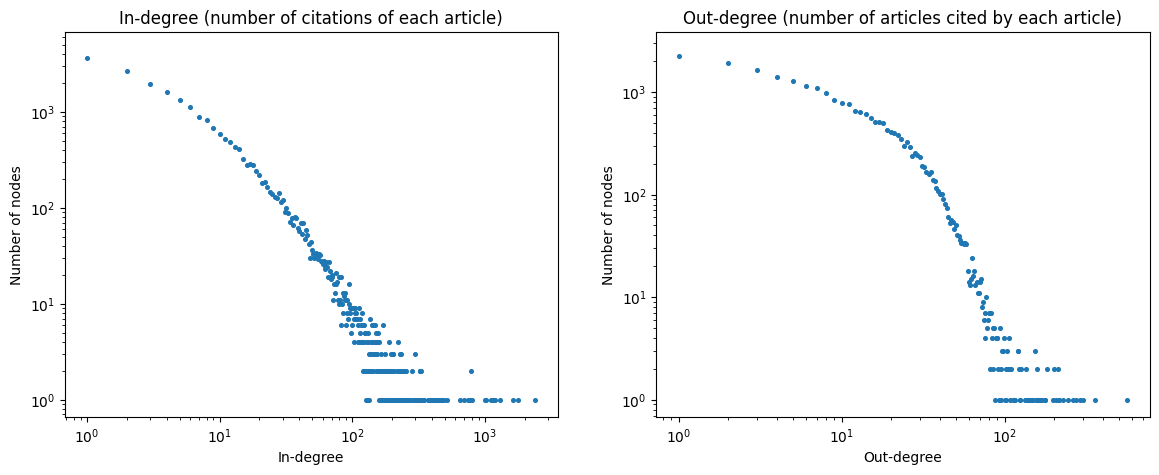
\includegraphics[width=1\linewidth]{degree_distribution.png}
\caption{Degrees distribution.}
\label{plot:degree}
\end{figure}

The first distribution is rather typical for a scale-free network and follows the power law. However, it is not exactly the case with the out-degree distribution. The possible explanation to this is the following: if we look at the graph as a temporal graph (we have dates of each paper's publishing) out-degree of each node is determined on creation and does not change over time. In-degree, on the other hand, has a behaviour that is much closer to how degrees act in a usual social graph, developing over time.

\subsection{Centralities}
\tab Centralities are characteristics of nodes that determine how "important" or "popular" each of them is. There are several types of them and each measures this "importance" in its own way. We will visualize distribution of three centralities.
\begin{itemize}
\item[a)] Eigenvector centrality. In general, relative scores are assigned to all nodes in the network based on the concept that connections to high-scoring nodes contribute more to the score of the node in question than equal connections to low-scoring nodes.
\begin{figure}[h]
\centering
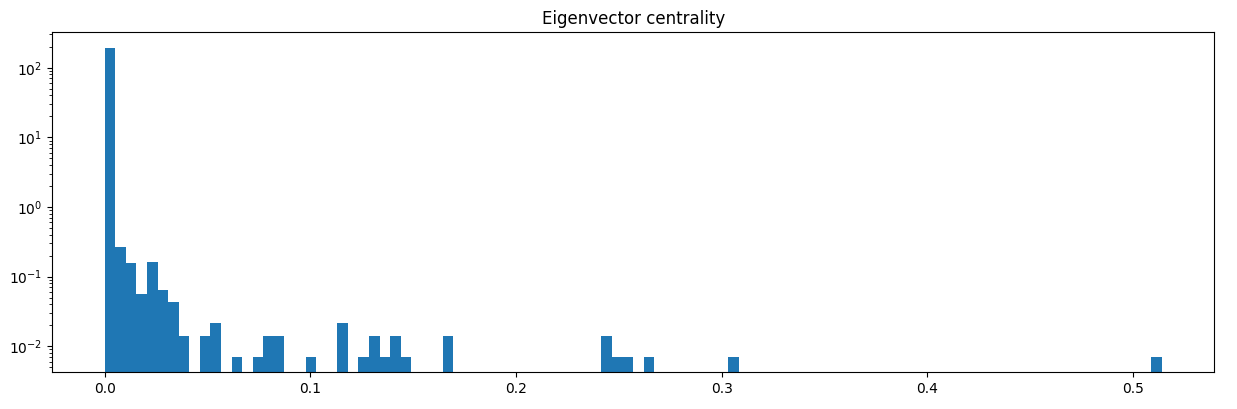
\includegraphics[width=1\linewidth]{centralities_eigenvector.png}
\caption{Eigenvector centrality distribution.} \label{plot:centrality:eigenvector}
\end{figure}
\item[b)] Closeness centrality. It is calculated as the reciprocal of the sum of the length of the shortest paths between the node and all other nodes in the graph. It measures how "close" the node is to the rest of the graph.
\begin{figure}[h]
\centering
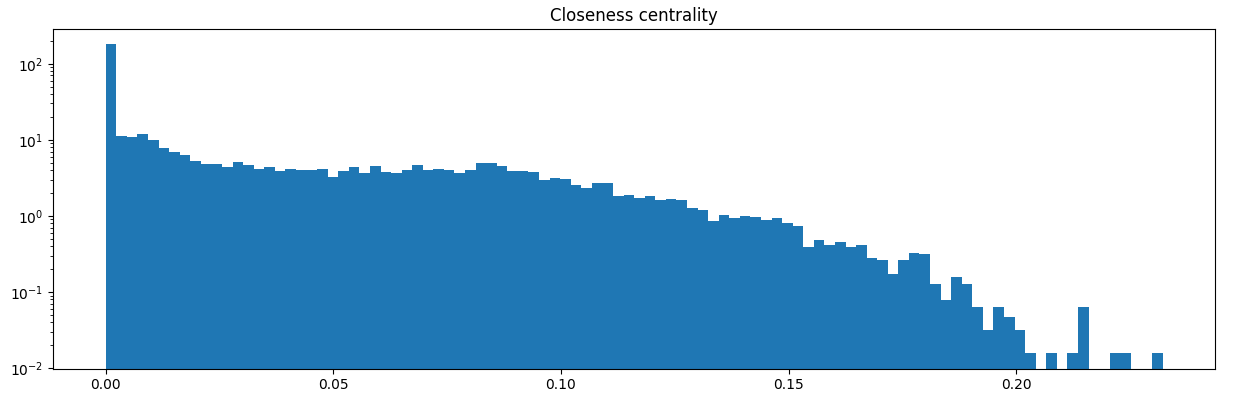
\includegraphics[width=1\linewidth]{centralities_closeness.png}
\caption{Closeness centrality distribution.} \label{plot:centrality:closeness}
\end{figure}
\item[c)] Betweenness centrality. The betweenness centrality for each node is the number of shortest paths that pass through this node. In other words, it determines whether the node is a hub.
\begin{figure}[h]
\centering
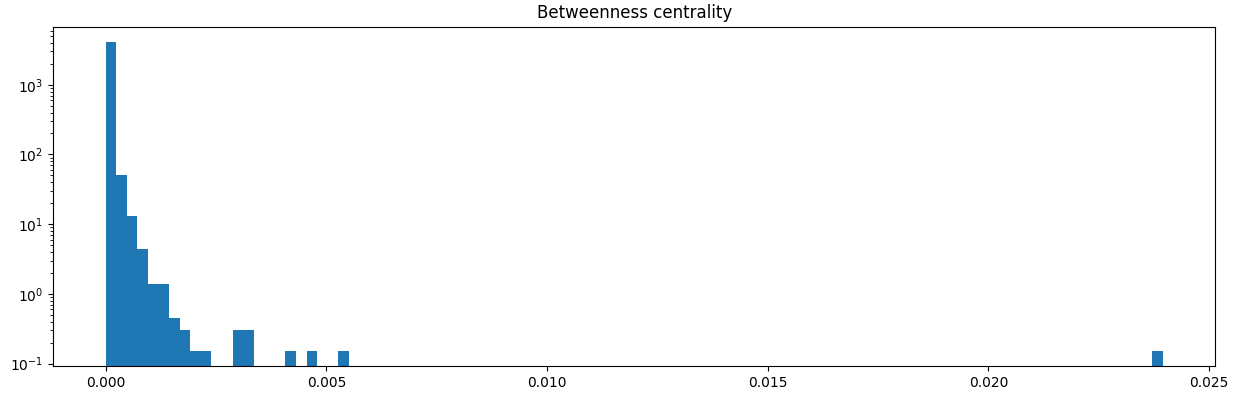
\includegraphics[width=1\linewidth]{centralities_betweenness.png}
\caption{Eigenvector centrality distribution.} \label{plot:centrality:betweenness}
\end{figure}
\end{itemize}

\subsection{Time Properties}
\tab Since our graph can be interpreted as a temporal graph, we can study the way its properties change over time. For instance, we discovered that the number of new papers per unit of time increases but the rate of the increase decreases. See Figure \ref{plot:number_of_new_papers} for the plots.
\begin{figure}[h]
\centering
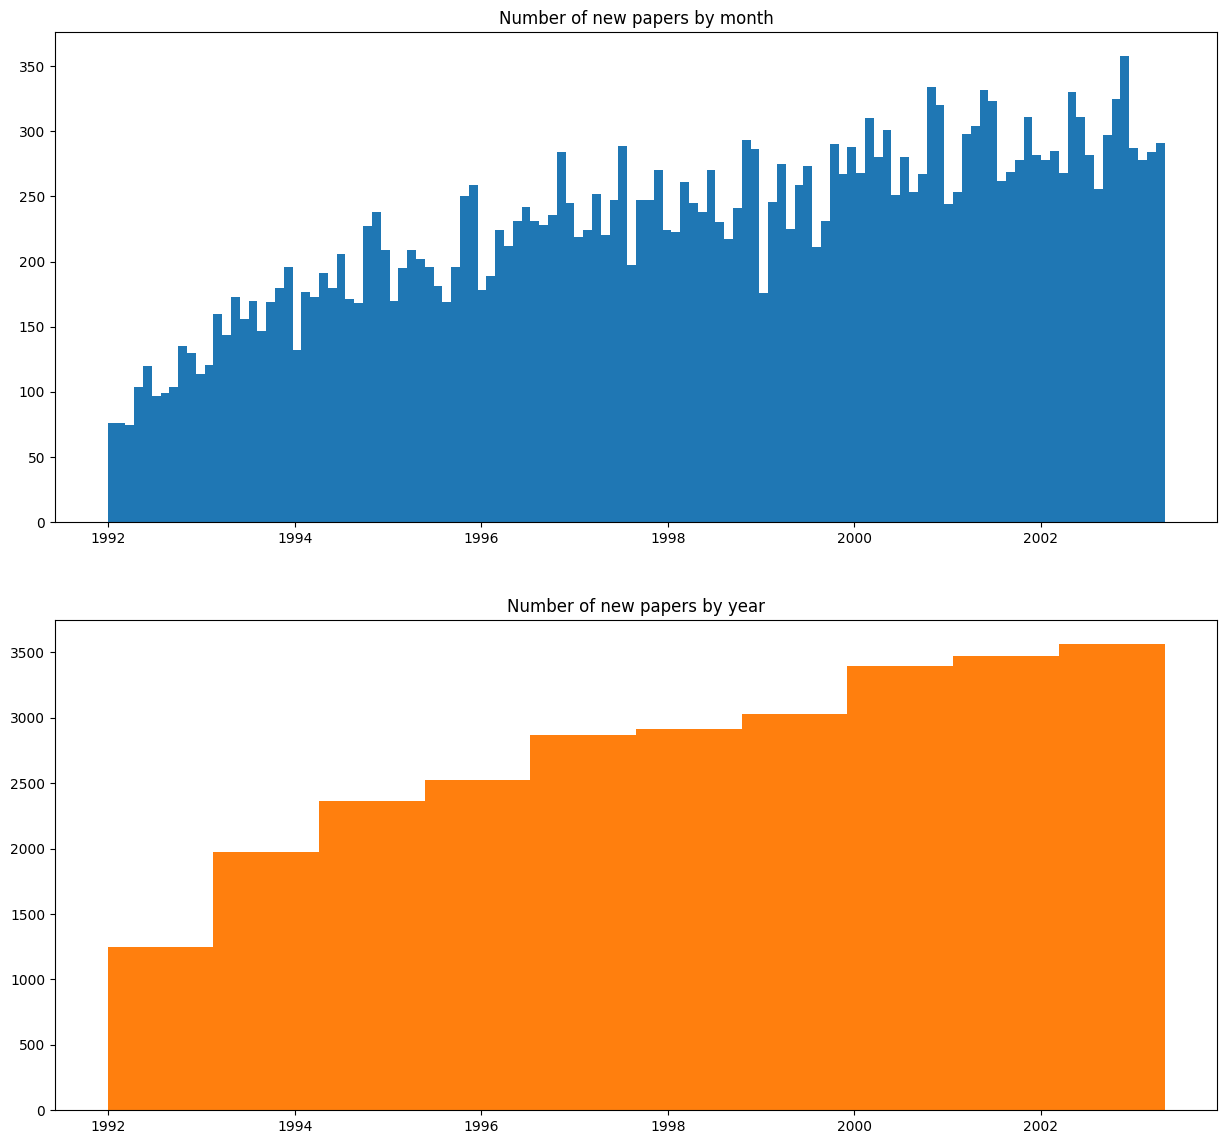
\includegraphics[width=0.9\linewidth]{new_papers_over_time.png}
\caption{Number of new papers published each two months and each year.}
\label{plot:number_of_new_papers}
\end{figure}

Another interesting thing that we found is how average in-degrees and out-degrees change (see Figure \ref{plot:average_degree_per_month}).
\begin{figure}[h]
\centering
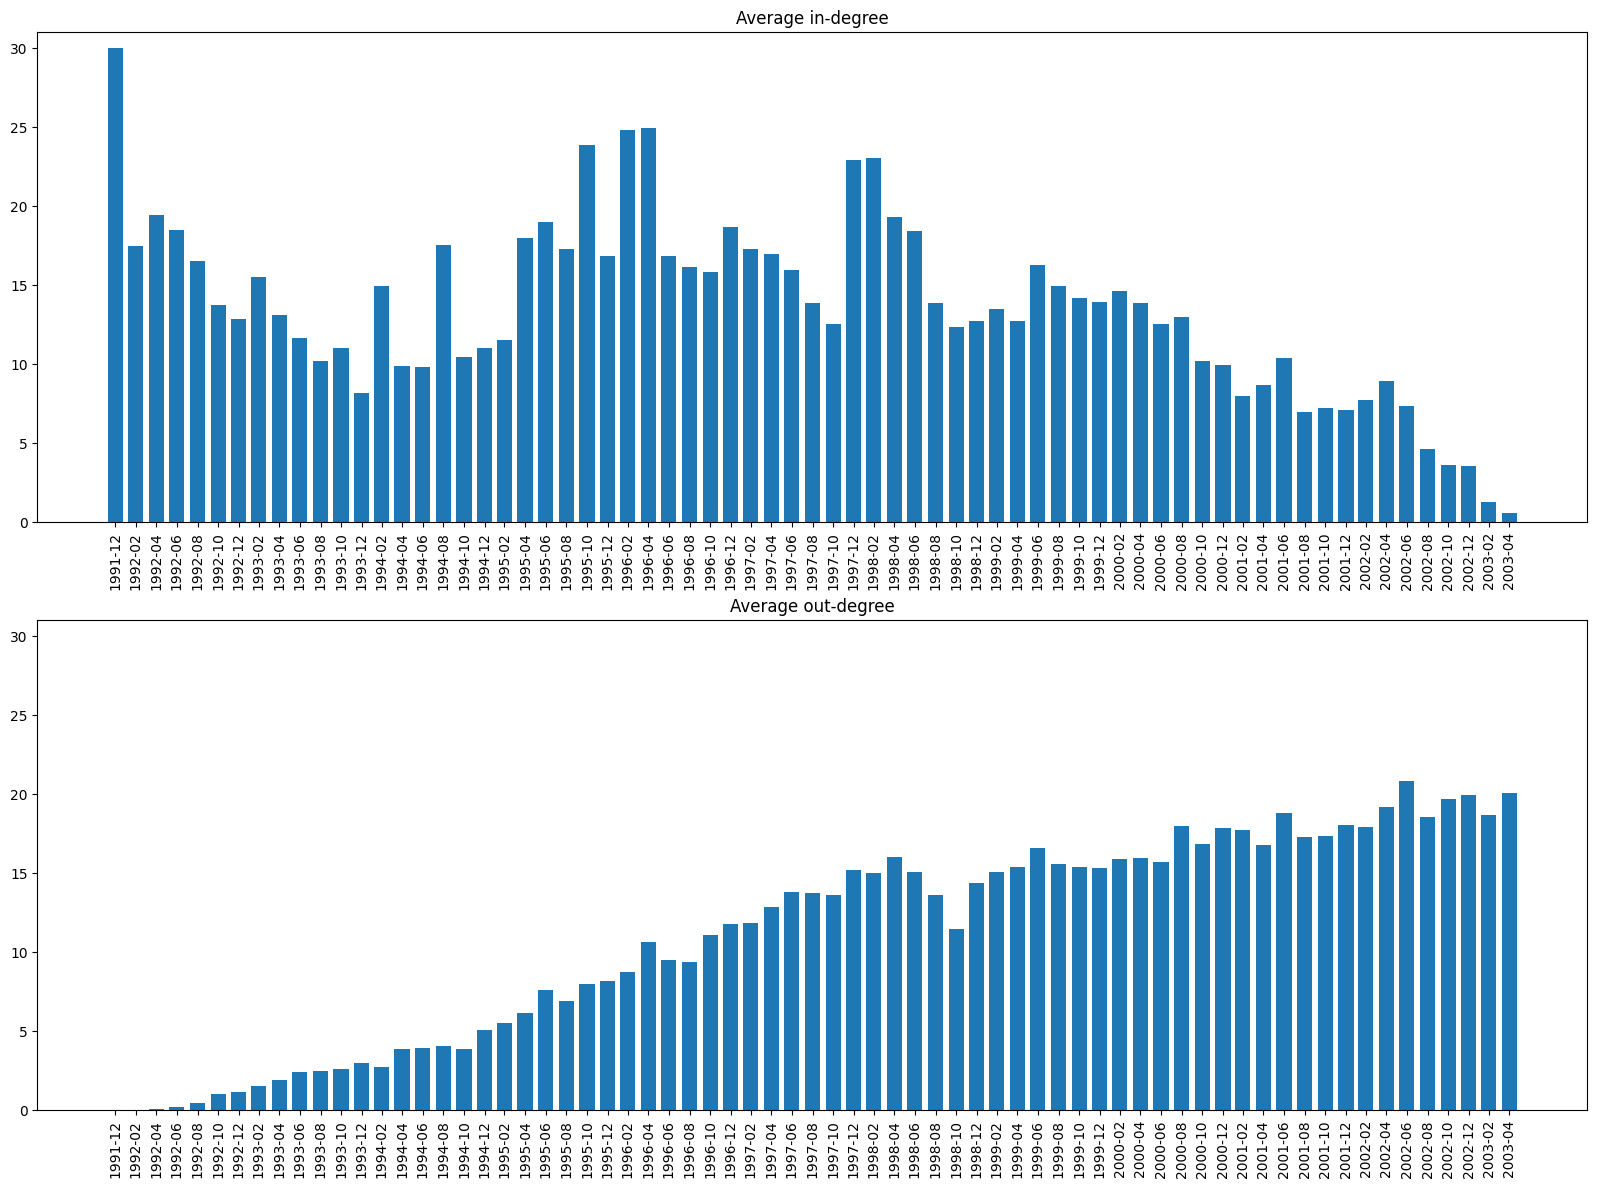
\includegraphics[width=1\linewidth]{degrees_over_time.png}
\caption{Average degrees in 2 months time from 1991 to 2003.} \label{plot:average_degree_per_month}
\end{figure}
A downwards trend in the end for in-degree and upwards trend in the beginning are noticeable. Explanation to this phenomena is rather simple: older papers had more time to gain popularity and therefore have more incoming edges, whereas papers from 2003 do not have any papers in our dataset that cite them. The opposite happens with the out-degree. Earlier papers cited even earlier papers (from 1980s) that were not included in our graph and thus have little to no outgoing edges. It is also worth noticing that the growth of out-degree slows down closer to 2003. It means that almost enough papers are included in the graph at that time to publish a paper sourcing only these modern papers in our dataset.

\subsection{Clusterization}
Due to the duality of our problem, clusterization can be done either using node features (mainly papers' abstracts) or considering the graph structure (which is usually called community detection). As a measure of quality of the partition $P$ of graph $G$ we have chosen the metric modularity, which for directed graphs is defined as
$$\textbf{Modularity}(G, P) = \frac{1}{|E|} \sum_{u, v \in V} \left[\left(A_{u, v} - \frac{d_{\text{out}}(u)\cdot d_{\text{in}}(v)}{|E|}\right)\cdot \delta_P(u, v)\right],$$
where $A$  is the adjacency matrix and $\delta_P(u, v)$ is defined as
$$\delta_P(u, v) =
\begin{cases}
1, & \text{if nodes } u \text{ and } v \text{ lie in the same community in pratition } P \\
0, & \text{otherwise}
\end{cases}.
$$ 

First we did community detection on the graph. We compared Louvain and label propagation community detection algorithms since most other methods were extremely slow and thus not suitable for our graph. The best modularity was achieved by Louvain algorithm with partition into 31 classes with fixed seed compared to 969 classes using label propagation. 

To do clusterixation we have divided the articles into the same number of clusters according to their abstracts using text embedding from `glove-wiki-gigaword-50` model (we averaged the embeddings of each word in the abstract) and KMeans algorithm. We also tried agglomerative clustering and Gaussian mixture. Modularity for all of them was really poor, which should not come as a surprise. Visualizations of resulting clustering can be found on Figures \ref{plot:clustering:agglomerative} and \ref{plot:clustering:gaussian_mixture}. The comparison of clustering algorithms can be seen in Table \ref{table:clusterization}.

\begin{figure}[h]
\centering
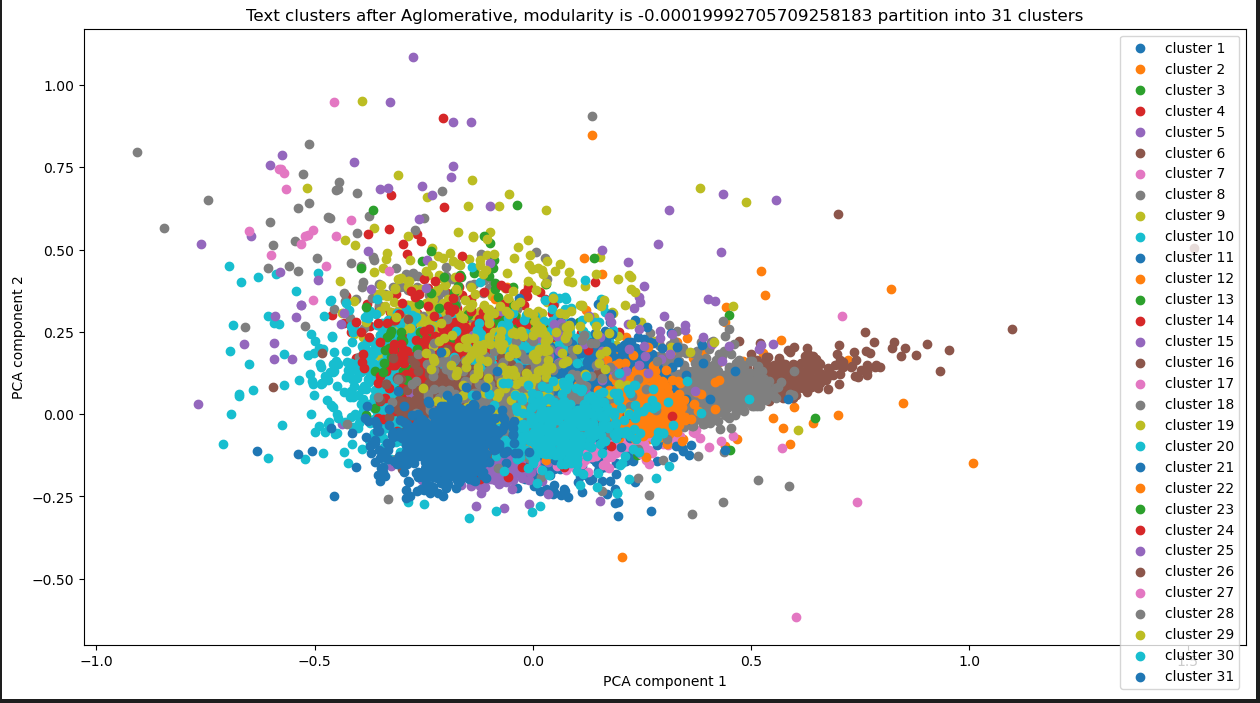
\includegraphics[width=1\linewidth]{Aglomerative.png}
\caption{Visualization of clustering using Agglomerative Clustering algorithm.}
\label{plot:clustering:agglomerative}
\end{figure}

\begin{figure}[h]
\centering
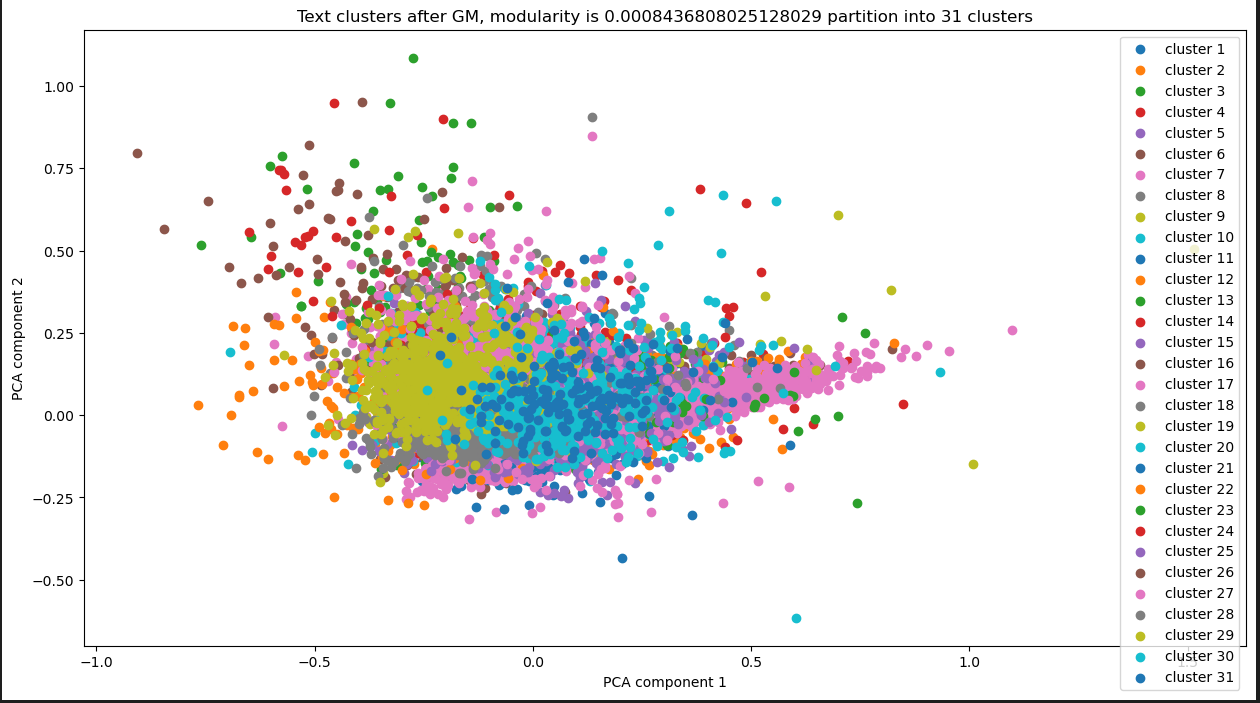
\includegraphics[width=1\linewidth]{gm.png}
\caption{Visualization of clustering using Gaussian Mixture model.}
\label{plot:clustering:gaussian_mixture}
\end{figure}

\begin{table}[h]
\centering
\begin{tabular}{c c c}
\hline\hline
Algorithm & Number of clusters & Modularity \\
\hline
Louvain & 31 & $0.655$ \\
Label Propagation & 969 & $0.541$ \\
Agglomerative Clustering & 31 & $-0.0002$ \\
Gaussian Mixture Model & 31 & $0.0008$ \\
\hline
\end{tabular}
\caption{Comparison of different clusterization algorithms.}
\label{table:clusterization}
\end{table}

\section{Methodology}
\subsection{Problem statement}
\tab Our main goal was to predict citation rates of the papers. We initially thought of solving a link prediction task (predicting the existence of edge between two nodes) since it seemed logical enough for our task. However, upon further considerations we eventually switched to node classifications. We classified citation rates into 4 classes using quartiles of in-degrees (this manner was inspired by scientific journals' tiers). This approach gave us even-ish distribution of classes. Note that the class boundaries are not evenly distributed, since our graph is a scale-free network.

To form target values and split our graph into train and test samples the following approach was used. Split the graph into two parts: all the nodes with publish date before 2001-01-01 (the date choice was arbitrary) and the rest of them, which will be referred to as old nodes and new nodes respectively. The new nodes have some edges into the old ones (new papers citing old papers), the number of which (converted into a class) for each old node was used as its target value. Note that the edges between old nodes were not considered in the target. By splitting old nodes into train and test sets we got our final data.

\subsection{Baseline}
\tab Before implementing any baseline we studied how other papers approached this problem. The state-of-the-art approach for baseline solutions, is to use some embedding method in combination with a simple regression or classification model(depending on the task). We used similar approach in out study

As a baseline model we employed logistic regression classifier as a classical model. We trained it on three different node embeddings:
\begin{enumerate}

\item[1.] Text embeddings. \newline
We tried two different approaches of getting text embeddings:
\begin{enumerate}
\item[a)] Text had been preprocessed using stemmer and stop words removal before applying bag of words vectorization.
\item[b)] Text embeddings were obtained by averaging the embedding of each word in the abstract using glove-wiki-gigaword model with an embedding size of 50
\end{enumerate}

\item[2.] Graph embeddings.\newline
We used the classic node2vec with default parameters, except that the dimension of the embedding space was 64 (instead of default 128)
\end{enumerate}

The results of these methods can be found in the Table \ref{table:baseline_metrics}

\begin{table}[h]
\centering
\begin{tabular}{c c  c c c}
\hline\hline
 & & \multicolumn{3}{c}{Metrics} \\
\cline{3-5}
Classification model & Embeddings & \multirow{2}{*}{Accuracy} & \multicolumn{2}{c}{F1 score} \\
 & & & Macro & Weighted \\
\hline
\multirow{3}{*}{Logistic Regression} & Text preprocessing + BoW & 0.46 & 0.38 & 0.45 \\
 & Text 2 & 0.44 & 0.16 & 0.27 \\
 & Graph & 0.53 & 0.33 & 0.43 \\
\hline
\end{tabular}
\caption{Baseline metrics.}
\label{table:baseline_metrics}
\end{table}

\subsection{Our solution}
In search of a better solution, we tried GCN and GCNwLinear models with different types of node embeddings: random embeddings (learnable), text/graph-only embeddings and their concatenation (we tried both to train them, and not). In addition, we went through the following parameters:
\begin{verbatim}
n_layers = 6
random_emb_size = 32
hidden_dim = 128
crop_df = False
tune_embs = True
add_reverse_edges = True
dropout=0.2
lr = 5e-4
node_emb_size = 64
\end{verbatim}
Each parameter speaks for itself except of \textbf{crop\_df} which is responsible for getting rid of the imbalance of classes in the dataset by removing some samples or not. Above you can see the best subset of this hyperparameters which gives the following metrics:
\begin{table}[h]
\centering
\begin{tabular}{c c  c c c}
\hline\hline
 & & \multicolumn{3}{c}{Metrics} \\
\cline{3-5}
Classification model & Embeddings & \multirow{2}{*}{Accuracy} & \multicolumn{2}{c}{F1 score} \\
 & & & Macro & Weighted \\
\hline
\multirow{1}{*}{GCNwLinear} & Concatenated text and node embs & 0.58 & 0.54 & 0.59 \\
\hline
\end{tabular}
\caption{Final metrics.}
\label{table:final_metrics}
\end{table}
\end{document}